\documentclass{article}
\usepackage[utf8]{inputenc}
\usepackage[english, ukrainian]{babel}
\usepackage{fontsize}
\usepackage{geometry}
\usepackage{amsthm}
\usepackage{amsfonts}
\usepackage{graphicx}
\usepackage[ruled]{algorithm2e}
\usepackage{hyperref}
\usepackage{biblatex}
\usepackage{csquotes}
\usepackage{mathtools}
\usepackage{amsmath}
\usepackage{amssymb}
\usepackage{bbm}
\usepackage{tabularx}
\usepackage{xcolor}

\usepackage{tikz}
\usetikzlibrary{decorations.pathmorphing}

\usepackage{enumitem}
\usepackage{nicefrac}

\usetikzlibrary{patterns}

\usepackage{diagbox}
\usepackage{longtable}

\usepackage{float}


\usepackage{enumitem}
\usepackage{nicefrac}

\usepackage{listings}
\definecolor{codegreen}{rgb}{0,0.6,0}
\definecolor{codegray}{rgb}{0.5,0.5,0.5}
\definecolor{codepurple}{rgb}{0.58,0,0.82}
\definecolor{backcolour}{rgb}{0.95,0.95,0.92}

\lstdefinestyle{mystyle}{
    backgroundcolor=\color{backcolour},   
    commentstyle=\color{codegreen},
    keywordstyle=\color{magenta},
    numberstyle=\tiny\color{codegray},
    stringstyle=\color{codepurple},
    basicstyle=\ttfamily\footnotesize,
    breakatwhitespace=false,         
    breaklines=true,                 
    captionpos=b,                    
    keepspaces=true,                 
    numbers=left,                    
    numbersep=5pt,                  
    showspaces=false,                
    showstringspaces=false,
    showtabs=false,                  
    tabsize=2
}

\lstset{style=mystyle}
\hypersetup{colorlinks=true, linkcolor=[RGB]{255, 3, 209}, citecolor={black}}

\graphicspath{ {../Images/} }

\begin{document}
    \begin{titlepage}
        \begin{center}
            \begin{center}
                НАЦІОНАЛЬНИЙ ТЕХНІЧНИЙ УНІВЕРСИТЕТ УКРАЇНИ
                «КИЇВСЬКИЙ ПОЛІТЕХНІЧНИЙ ІНСТИТУТ імені Ігоря СІКОРСЬКОГО»

                Фізико-технічний інститут
            \end{center}
        $\newline$
        \vspace{3.3cm}
        
        {
        РОЗРАХУНКОВО-ГРАФІЧНА РОБОТА
        на тему:
        "Використання клітинних автоматів та генетичного алгоритму для "генерації" або "викривлення" музики"

        }
        \vspace{3cm}
        \begin{flushright}
            Виконав\\студент 3 курсу ФТІ\\групи ФІ-21\\Климентьєв Максим Андрійович
            
            \vspace{1cm}

            Перевірив:\\\underline{\hspace{5cm}}\\Оцінка:\\\underline{\hspace{5cm}}
        \end{flushright}
        \vspace{3.5cm}
        Київ --- 2025
        \end{center}
    \end{titlepage}
    \newpage

    \pagenumbering{gobble}
    \tableofcontents
    \cleardoublepage
    \pagenumbering{arabic}
    \setcounter{page}{3}

    \newpage
    \section{Актуальність теми}
    Можливість генерації музики за допомогою клітинних автоматів та генетичного алгоритму є актуальною, оскільки вони можуть дати натхнення, якого може не завжди вистачати, дозволяючи створювати унікальні музичні фрагменти, експериментувати зі звуком та ритмом.

    \section{Конкретизована мета роботи}
    Метою роботи є створення програмних реалізацій клітинного автомату та генетичного алгоритму для генерації або викривлення музики. Зокрема, ставиться завдання автоматичної побудови послідовності нот та їх обробки з метою створення музичних варіацій.

    \section{Обґрунтування методів обробки}
    Клітинні автомати, такі як "Game of Life", Rule 110 чи Brian's Brain, здатні породжувати складні структури на основі простих правил. Їхнє використання для генерації музики дозволяє створювати унікальні шаблони мелодії.  
    Генетичні алгоритми, з іншого боку, дозволяють "еволюціонувати" музику на основі фітнес-функції — наприклад, відповідності гармоніям або ритмам, заданим користувачем. Вони імітують біологічний відбір, використовуючи кросовери та мутації для оптимізації музичних фраз.

    \section{Розробка програмного забезпечення та виконання обробки даних}
        Було реалізовано два основних модулі та інтерфейс для взаємодії з ними:
        \begin{itemize}
            \item Модуль клітинного автомату, який генерує набір чисел, що інтерпретуються як висоти звуку.
            \item Модуль генетичного алгоритму, який працює з MIDI-послідовностями: проводить селекцію, схрещування та мутацію, щоб створити нову варіацію на основі заданої мелодії.
        \end{itemize}
        \begin{figure}[h!]
            \centering
            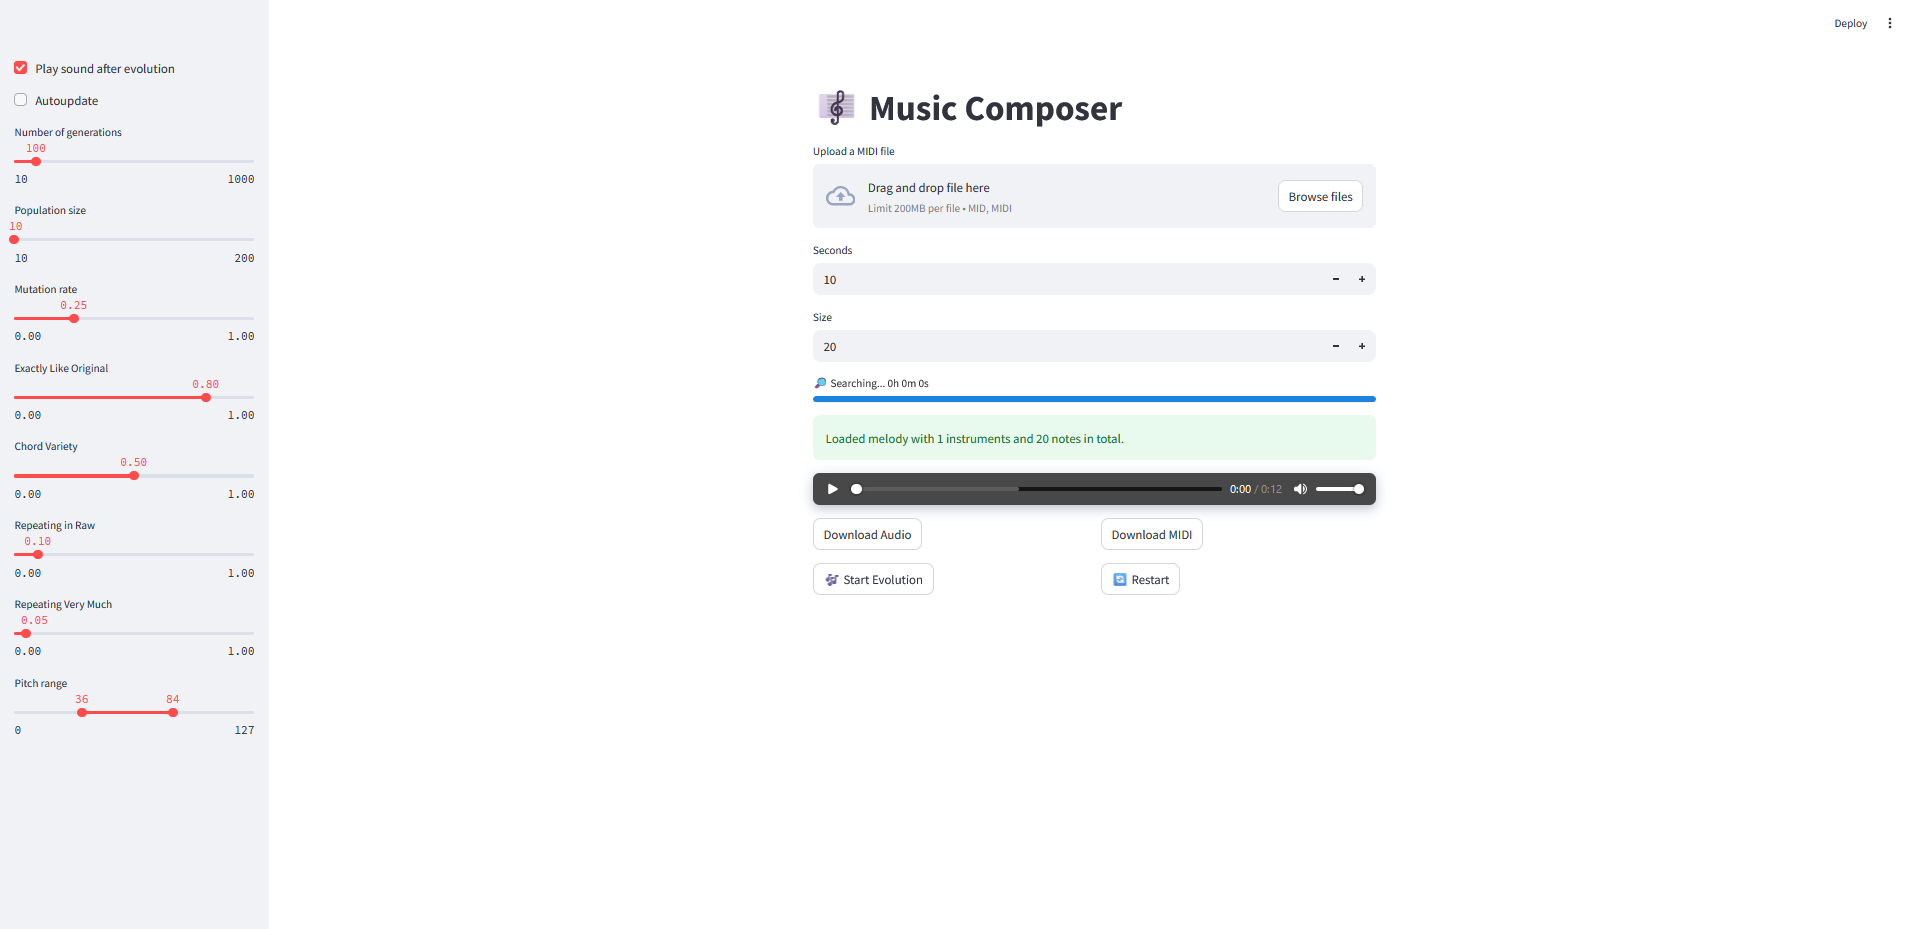
\includegraphics[width=0.9\linewidth]{upload.png}
        \end{figure}
        \begin{figure}[h!]
            \centering
            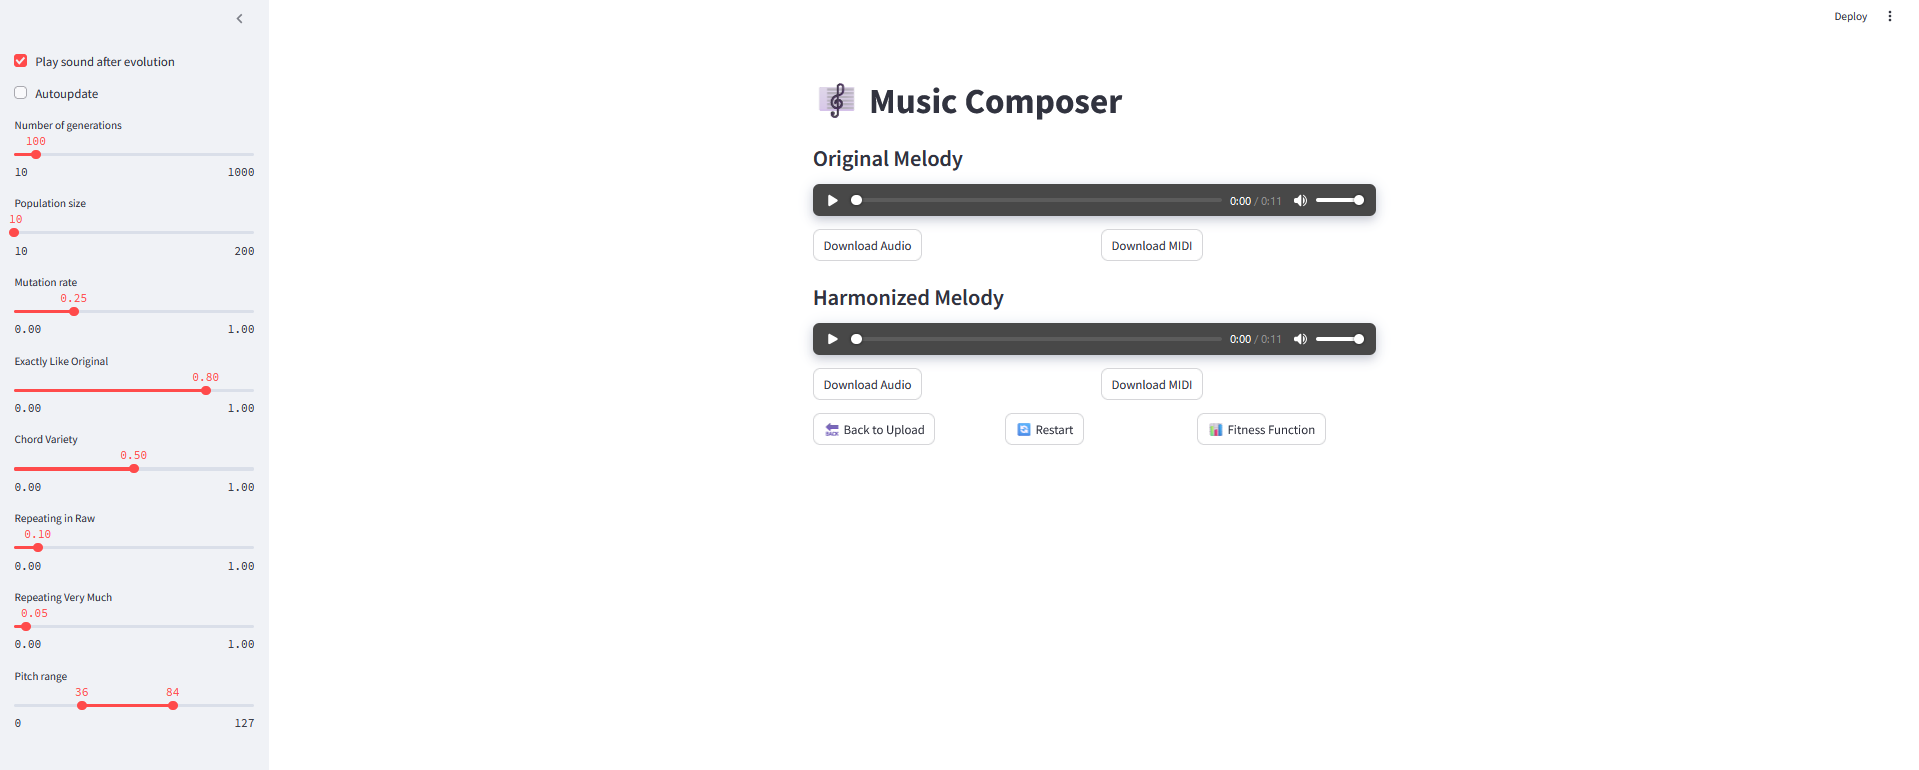
\includegraphics[width=0.9\linewidth]{results.png}
        \end{figure}
        \begin{figure}[h!]
            \centering
            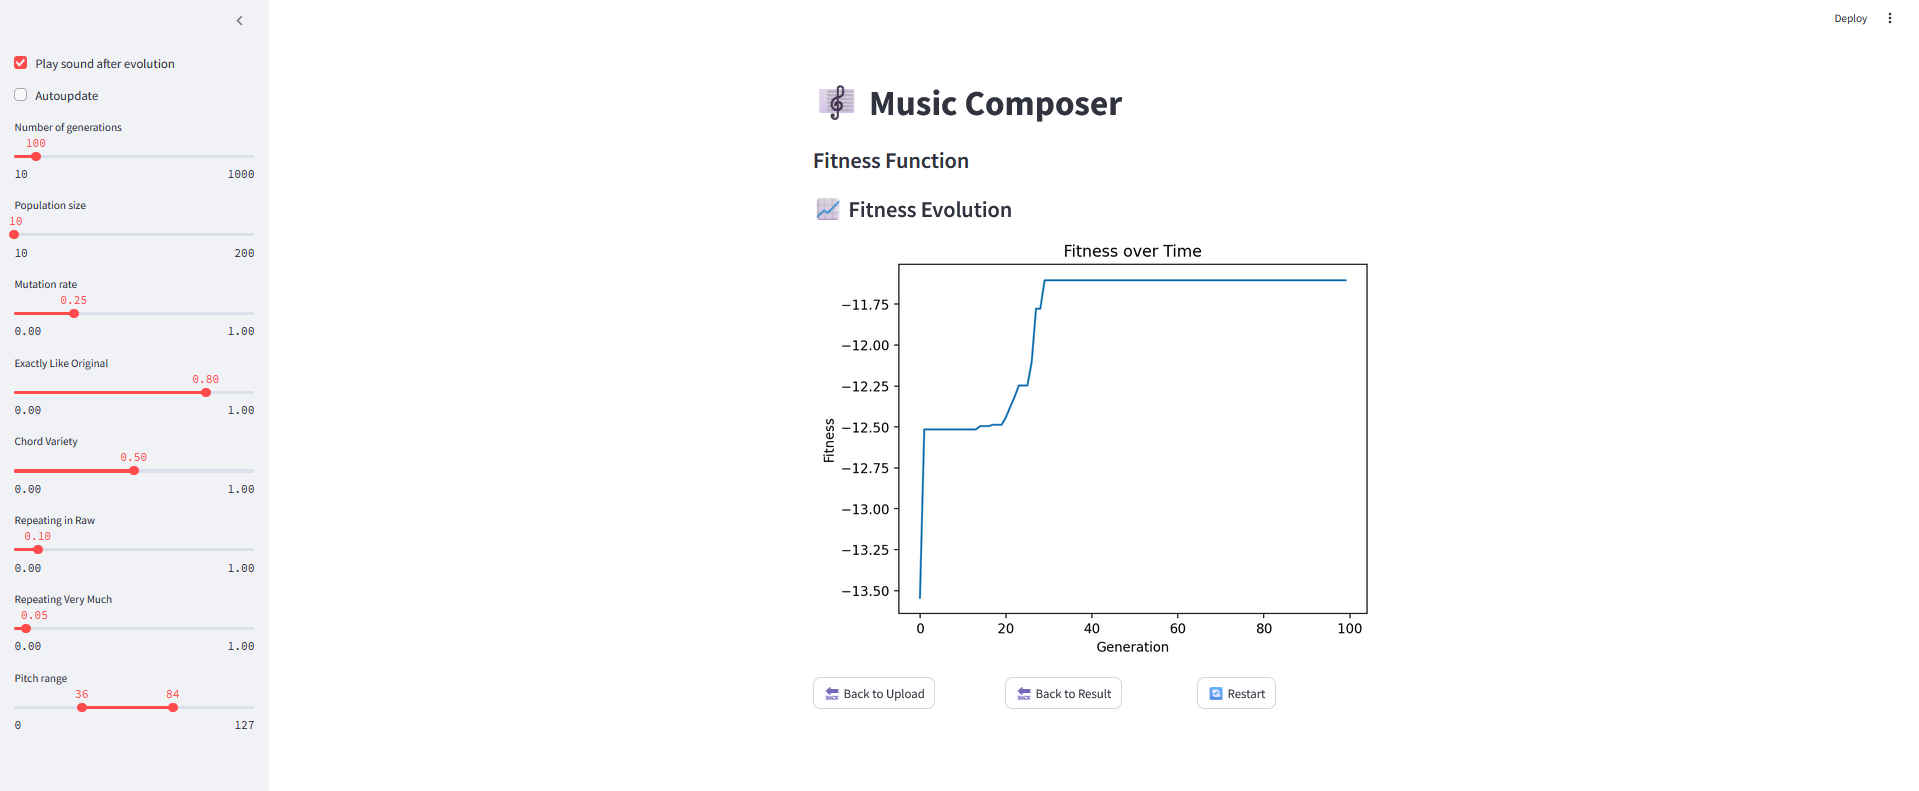
\includegraphics[width=0.9\linewidth]{fitness.png}
        \end{figure}

    \section{Представлення та систематизація результатів}
        Результати демонструються у вигляді:
        \begin{itemize}
            \item Побудови MIDI-файлів, які можна прослухати або вивантажити.
            \item Статистики фітнес-функції протягом еволюційного процесу.
        \end{itemize}
        Були створені кілька варіантів музичних фрагментів, які демонструють здатність алгоритмів створювати музичне різноманіття та структуру.
    

    \section{Висновки}
        У результаті виконаної роботи:
        \begin{itemize}
            \item Реалізовано клітинний автомат, який генерує нетипову музику.
            \item Розроблено генетичний алгоритм, здатний змінювати (викривляти) музичні послідовності з урахуванням певних критеріїв.
            \item Створено інтерфейс для візуалізації та прослуховування результатів.
        \end{itemize}

    \section{Список літератури}
        \begin{enumerate}
            \item Голуб Михайло
            \item \url{https://youtu.be/YoRPjU_Fbq0?si=N1BBvR2WYfsGIaQ0}
            \item \url{https://youtu.be/GIoLWVPb8mc?si=0POzxkd5j0PYJ7ct}
            \item \url{https://youtu.be/CAVy7OZ87mE?si=mhDH6eNMUXvBTX_A}
            \item \url{https://youtu.be/AmtLrd-cYSY?si=ZphdlqcWBmK6wYNc}
        \end{enumerate}
\end{document}
